\documentclass[a4j]{ujarticle}
\usepackage[dvipdfmx]{graphicx}
\usepackage{url}
\usepackage{bbding}
\usepackage{lscape}
\usepackage[subrefformat=parens]{subcaption}
\usepackage{bm}
\usepackage{amsmath}

\title{進捗報告資料}
\author{安達智哉\\to-adachi@ist.osaka-u.ac.jp}
\date{2019年4月3日}

\begin{document}
\maketitle



\section{UEの状態遷移に伴う、シグナリングの発生数の調査}
\subsection{先行研究~1}
RRC Connected Inactive及びRRC Suspendedに関して述べられている、文献\cite{RRCStateHandlingfor5G}では、UEがConnected状態へ遷移する際に発生するシグナリング数は表\ref{table:signalings}ようになると述べられている。
RRC Suspended 状態ではUEのコンテキストの一部がUE及びネットワークに保持されているため、シグナリング数が減少している。
また、RRC Connected Inactive 状態では、RAN-コアネットワーク間の接続がkeep aliveとなっているため、RAN-コアネットワーク間のシグナリングは発生せず、UE-RAN間のシグナリングのみが発生する。
\begin{table}[htbp]
  \centering
  \caption{Signaling Overhead}
  \label{table:signalings}
  \begin{tabular}{ccccc}
    \hline
    遷移元                  & 遷移先              & \multicolumn{3}{c}{シグナリング数} \\
                            &                     & 無線      & S1     & S11     \\ \hline \hline
    Idle                    & Connected           & 9         & 3      & 2       \\
    RRC Suspended           & Connected           & 5         & 2      & 2       \\
    RRC Connected Inactive  & Connected           & 4         & 0      & 0       \\ \hline
  \end{tabular}
\end{table}

この文献\cite{RRCStateHandlingfor5G}では、IdleとRRC Suspended に関するシグナリング数に対しては、3GPPの仕様書\cite{3gpp.23.720}を根拠として示している。
文献\cite{3gpp.23.720}に示されている図を図\ref{Legacy_connection_setup}及び図\ref{Resumption_of_a_previously_suspended_RRC_connection}に示す。
これらの図を見ることによって、表\ref{table:signalings}に示されているシグナリング数を確認することが可能である。
また、MMEが処理するべきシグナリング数(MMEが送受信するシグナリング数)は、Idle及びRRC Suspendedそれぞれにおいて5個、4個であることがわかる。
しかし一方で、RRC Connected Inactive に関するシグナリング数に対しては参考文献を示していなかった。
\begin{figure}[htbp]
  \centering
  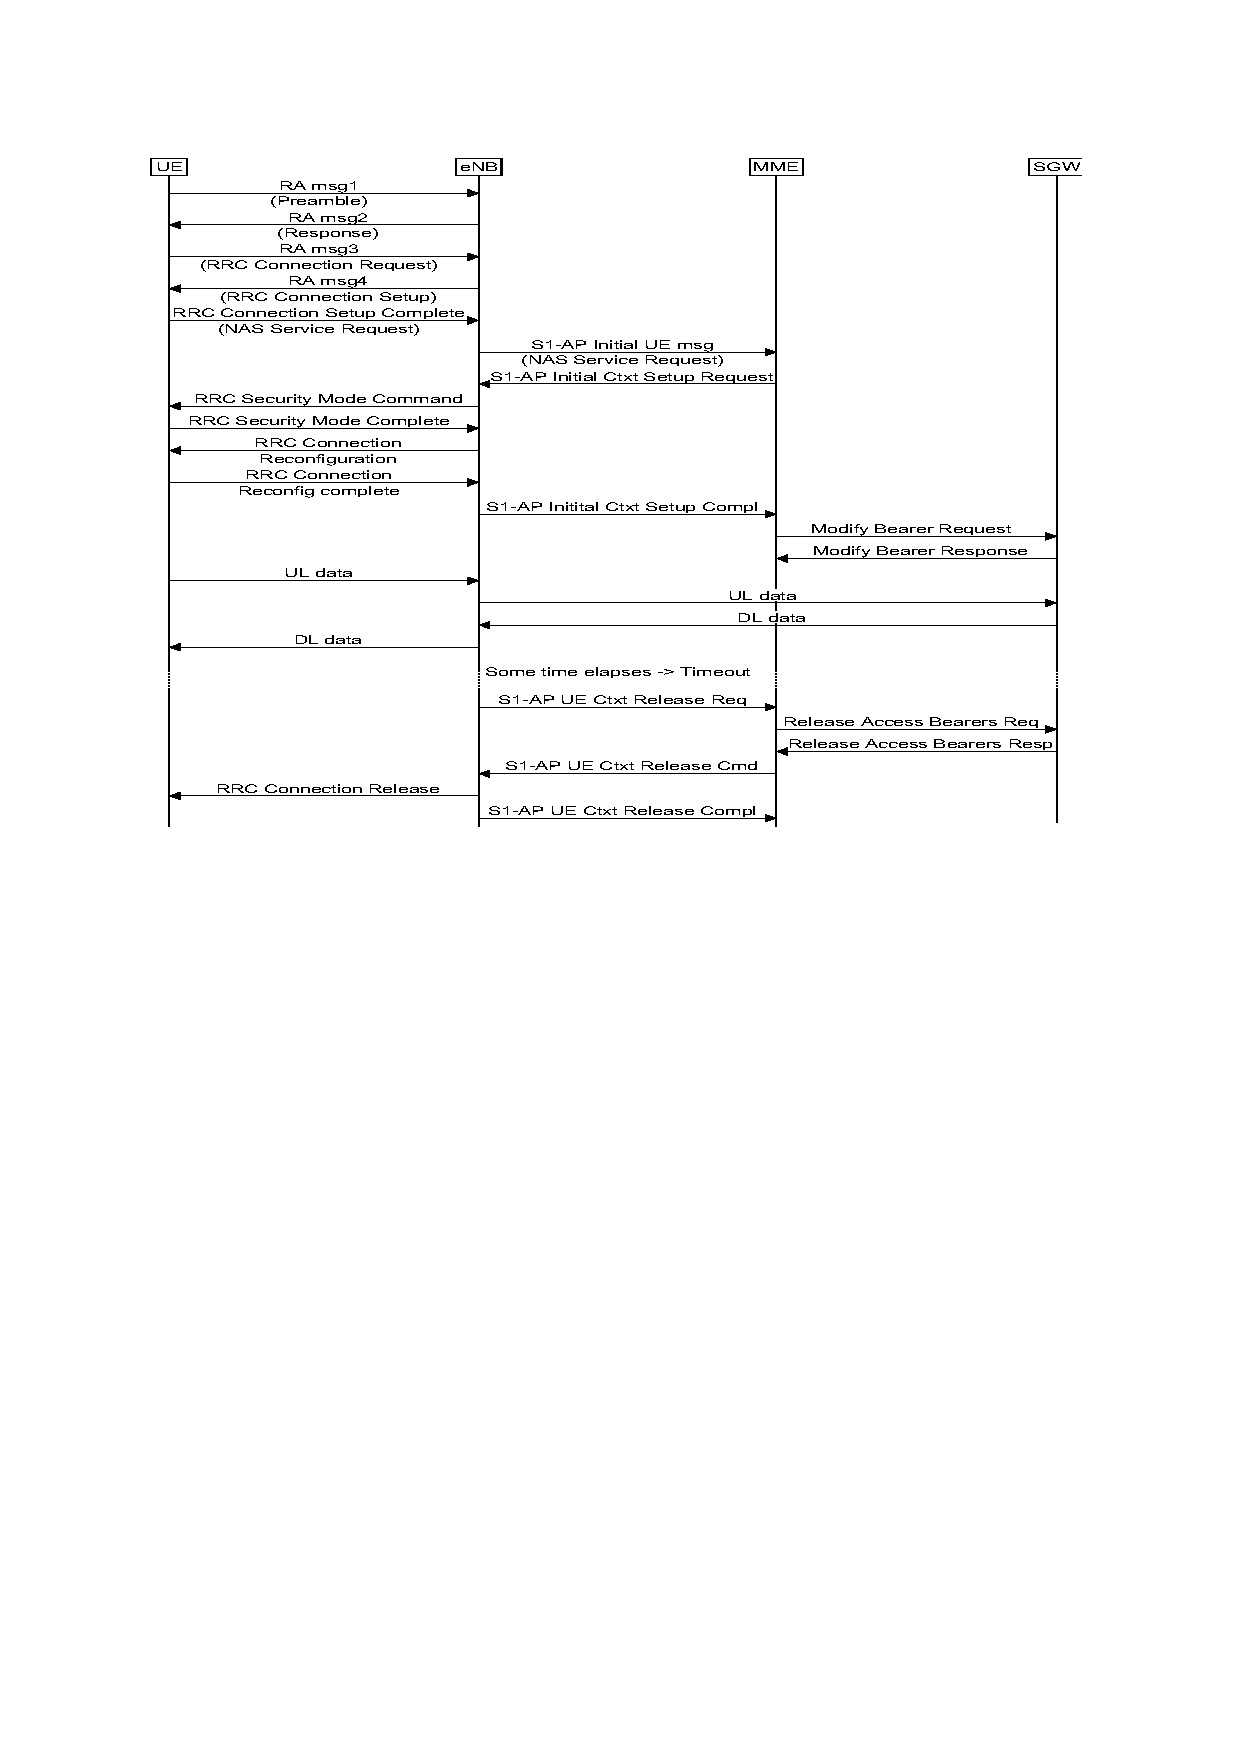
\includegraphics[width=0.9\hsize]{Legacy_connection_setup.pdf}
  \caption{Legacy connection setup}
  \label{Legacy_connection_setup}
\end{figure}

\begin{figure}[htbp]
  \centering
  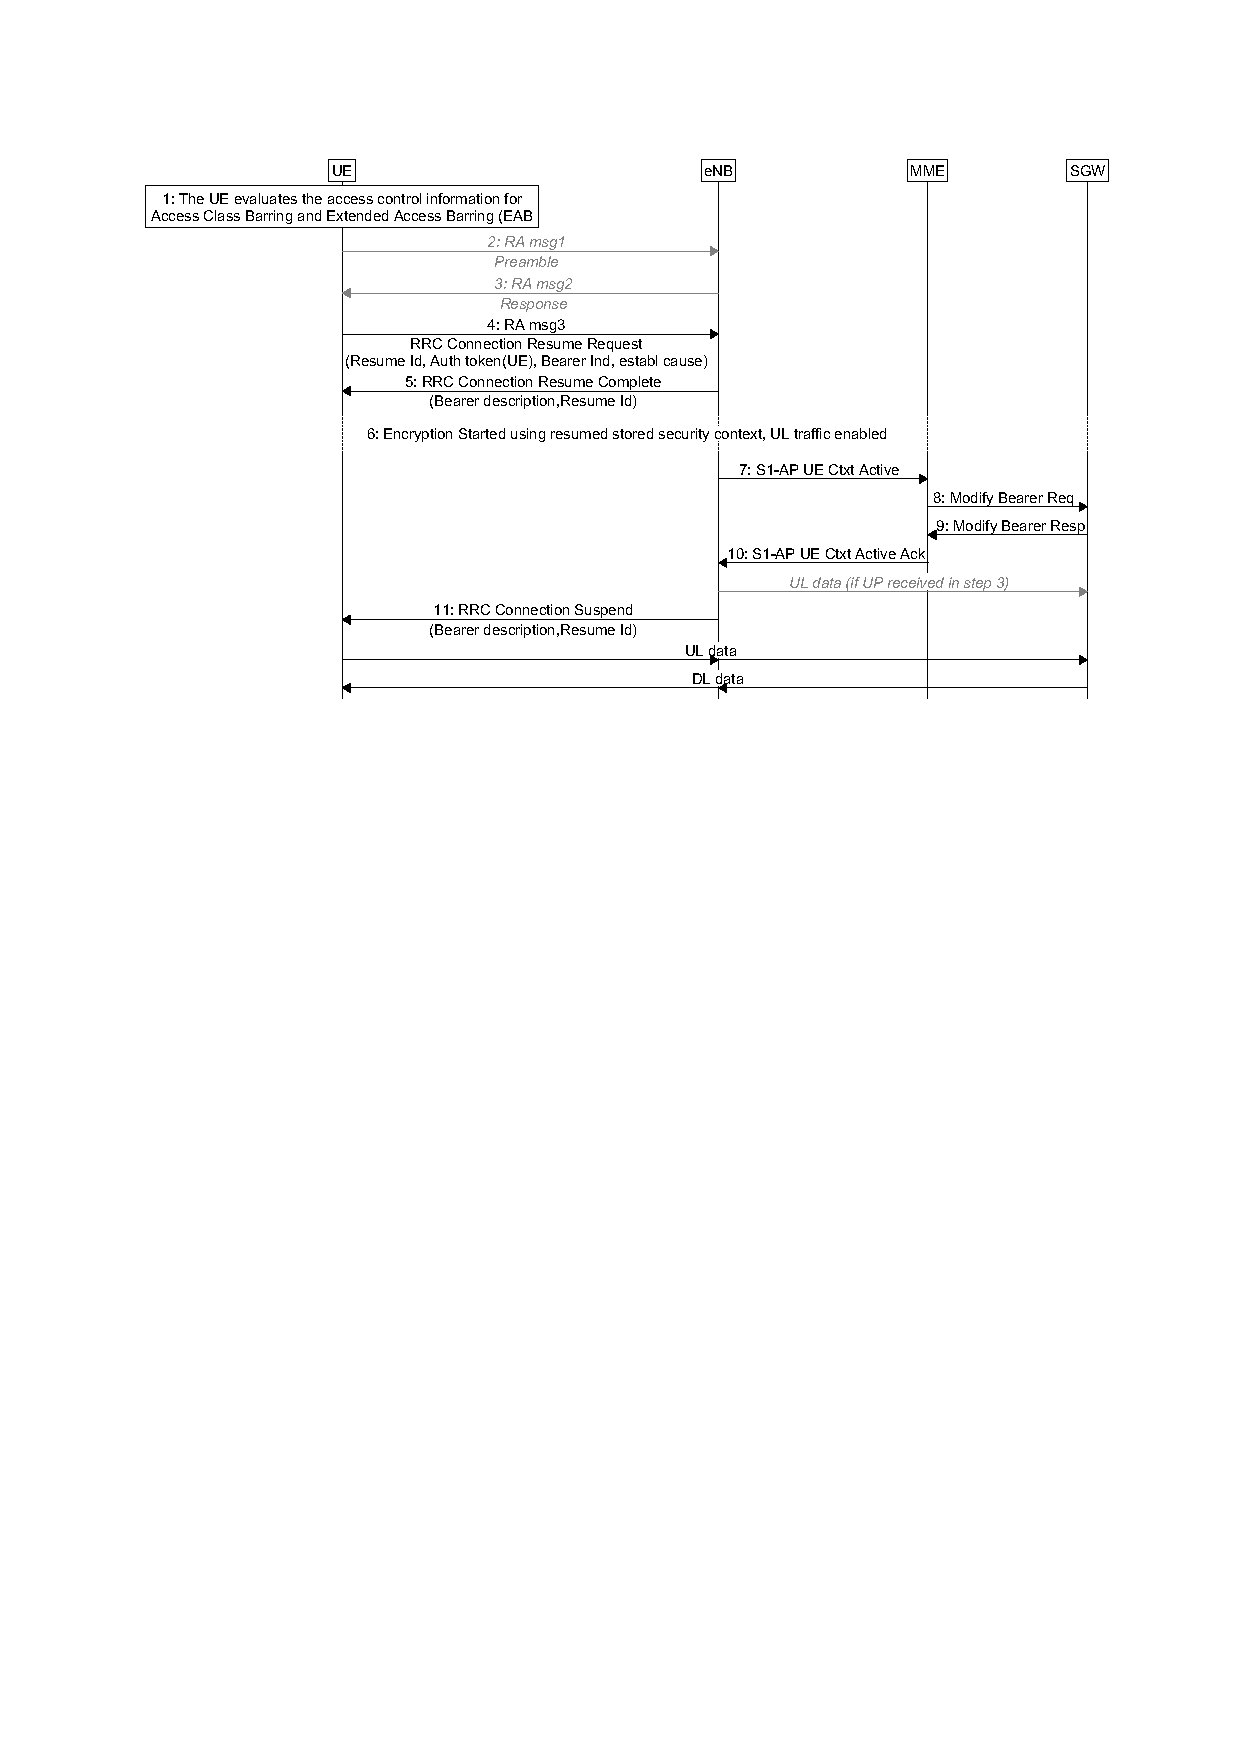
\includegraphics[width=0.9\hsize]{Resumption_of_a_previously_suspended_RRC_connection.pdf}
  \caption{Resumption of a previously suspended RRC connection}
  \label{Resumption_of_a_previously_suspended_RRC_connection}
\end{figure}

\clearpage
\subsection{先行研究~2}
文献\cite{ANovelStateModelfor5GRadioAccessNetworks}では、RRC Connected Inactive 状態からConnected状態へ遷移する際のシグナリング図を示していた。
そのシグナリング図を図\ref{Signaling_for_the_RRC_CONNECTED_INACTIVE_to_RRC_CONNECTED_transition_for_the_novel_state_model}に示す。
図\ref{Signaling_for_the_RRC_CONNECTED_INACTIVE_to_RRC_CONNECTED_transition_for_the_novel_state_model}を見ると、UE-RAN間のシグナリングが5回発生していることがわかる。
また、コアネットワーク側にはシグナリングは発生していないこともわかる。

\begin{figure}[htbp]
  \centering
  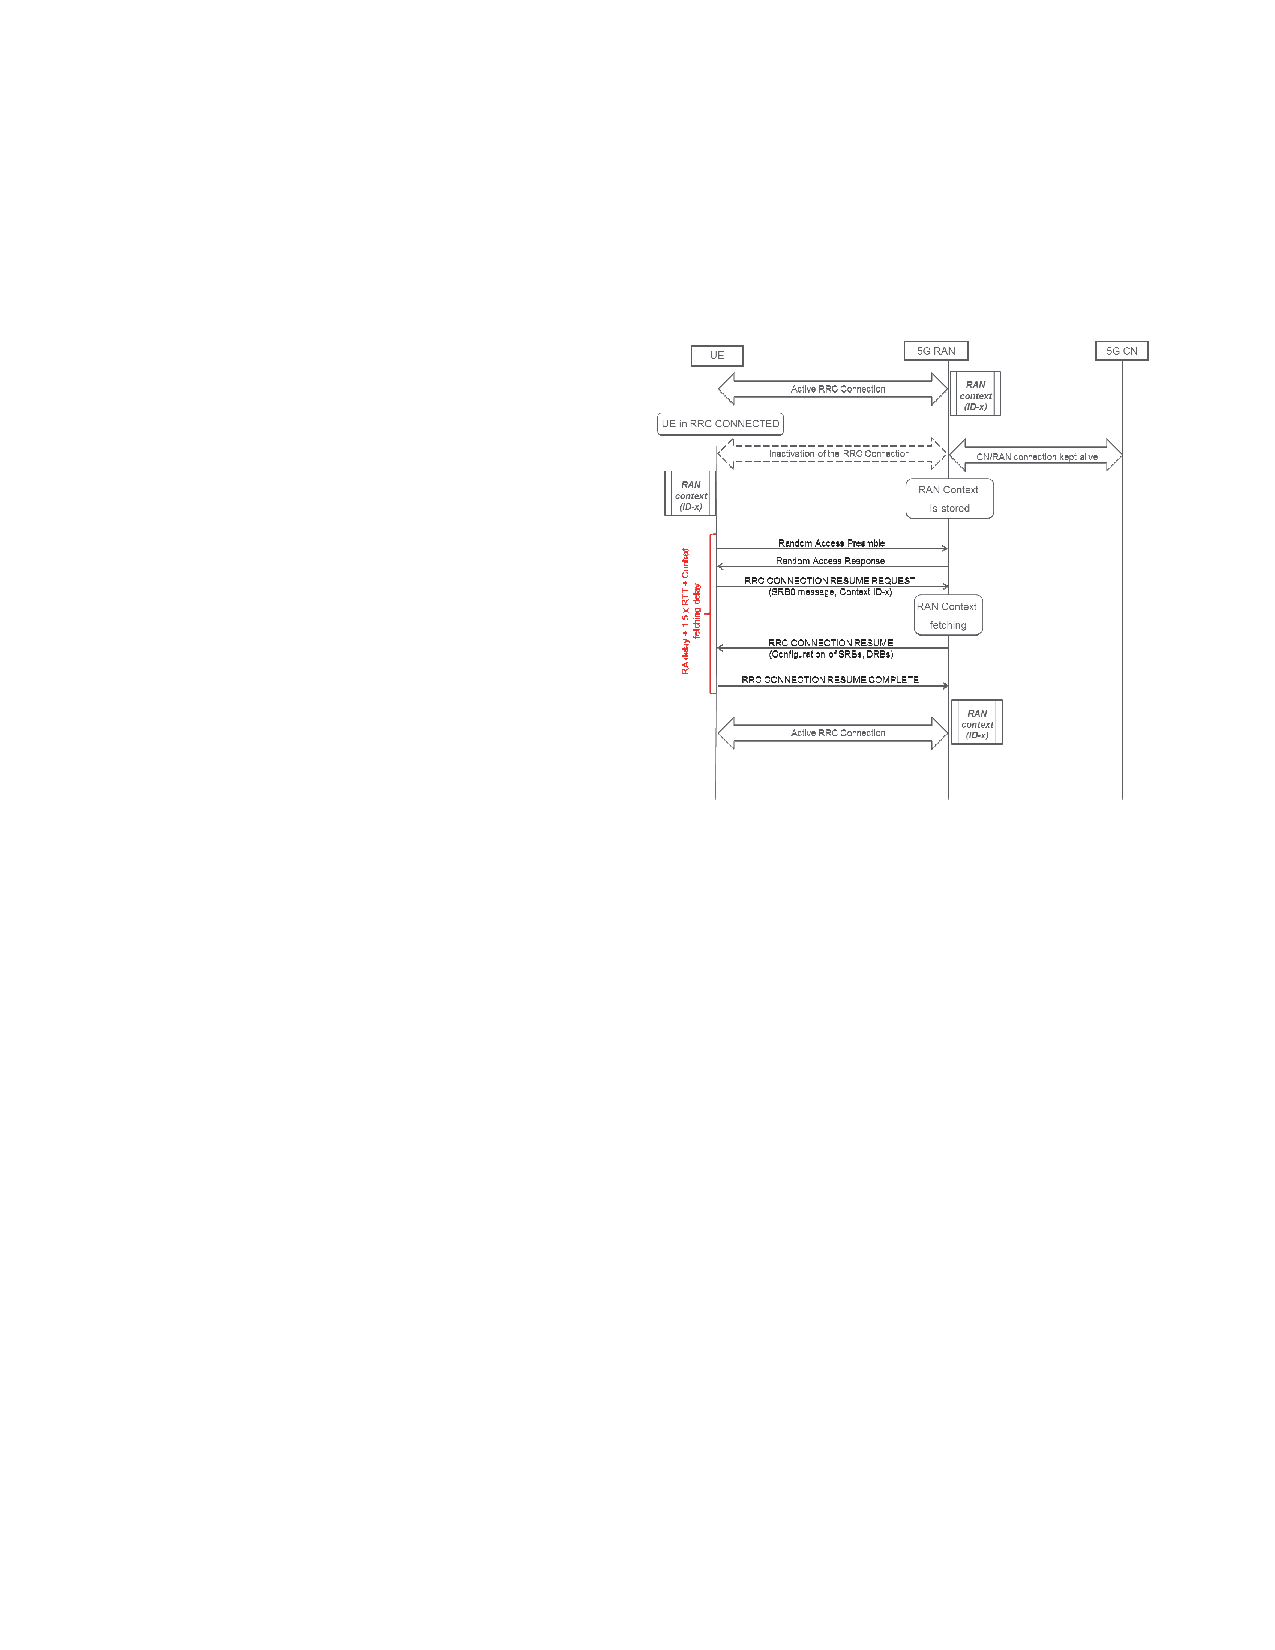
\includegraphics[width=0.9\hsize]{Signaling_for_the_RRC_CONNECTED_INACTIVE_to_RRC_CONNECTED_transition_for_the_novel_state_model.pdf}
  \caption{Signaling for the RRC CONNECTED INACTIVE to RRC CONNECTED transition for the novel state model}
  \label{Signaling_for_the_RRC_CONNECTED_INACTIVE_to_RRC_CONNECTED_transition_for_the_novel_state_model}
\end{figure}

\clearpage
\subsection{シグナリング数のまとめ}
先行研究を調査することにより、状態遷移に伴うシグナリングの発生数が一部であるが、明らかになった。
図\ref{state_id}に示す状態遷移図と共に、状態遷移に伴って発生するシグナリングに関する情報を、表\ref{table:signalings_all}に示す。

\begin{figure}[htbp]
  \centering
  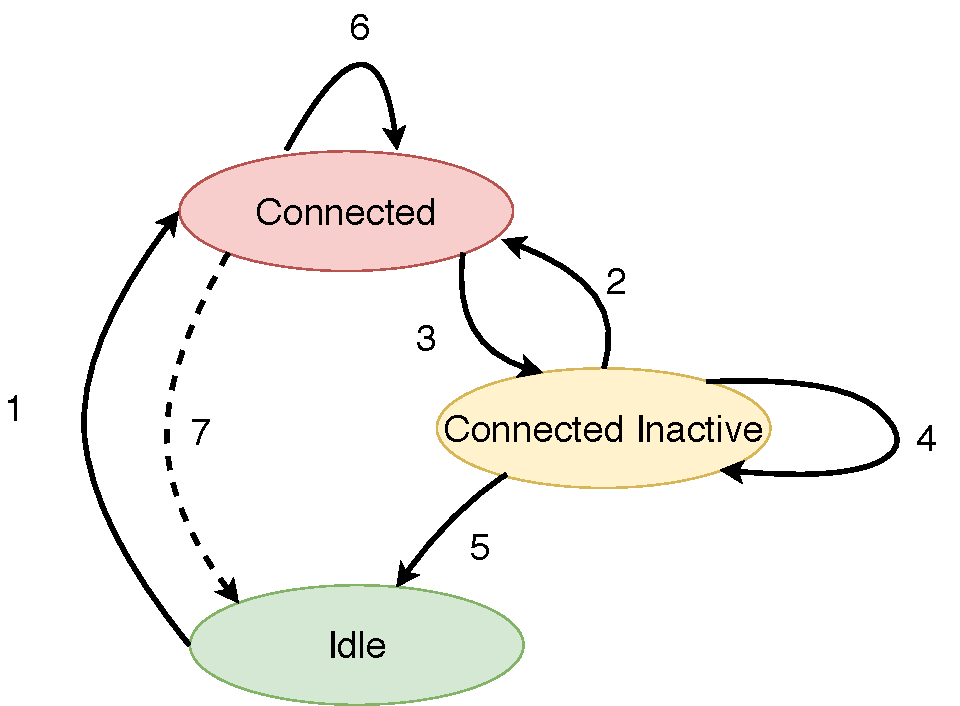
\includegraphics[width=0.9\hsize]{state_id.pdf}
  \caption{state transition}
  \label{state_id}
\end{figure}

\begin{table}[htbp]
  \centering
  \caption{Signaling Load}
  \label{table:signalings_all}
  \begin{tabular}{c|cccc|l}
    \hline
    遷移ID  & \multicolumn{4}{|c|}{シグナリング処理数} & 遷移条件                          \\
            & UE      & RAN     & MME     & SGW      &                                   \\ \hline \hline
    1       & 9       & 12      & 5       & 2        & Packets transmission              \\
    2       & 5       & 5       & 0       & 0        & 2 or more packets transmission    \\
    3       & ?       & ?       & ?       & ?        & Connected timer expiration        \\
    4       & ?       & ?       & ?       & ?        & One packet transmission           \\
    5       & ?       & ?       & ?       & ?        & Idle timer expiration             \\ \hline
  \end{tabular}
\end{table}

% \begin{itemize}
%   \item Idel
%   \item
%   \item
%   \item
% \end{itemize}



\section{今後の課題}
  \begin{itemize}
    \item 状態遷移に伴って発生するシグナリングの調査を継続する。
  \end{itemize}

\section*{\addcontentsline{toc}{section}{参考文献}}
\bibliographystyle{IEEEtran}
\bibliography{/Users/t-adachi/Documents/study/Bibliography/bib/hpt_core_network/myBib/LABbiblio,/Users/t-adachi/Documents/study/Bibliography/bib/hpt_core_network/Study_Group_Bibtex/bib/hptCoreNetwork_Study}
\end{document}
